\documentclass[border=10pt]{standalone}
\usepackage{tikz}
\usepackage{amsmath}
\usetikzlibrary{arrows.meta}

\begin{document}
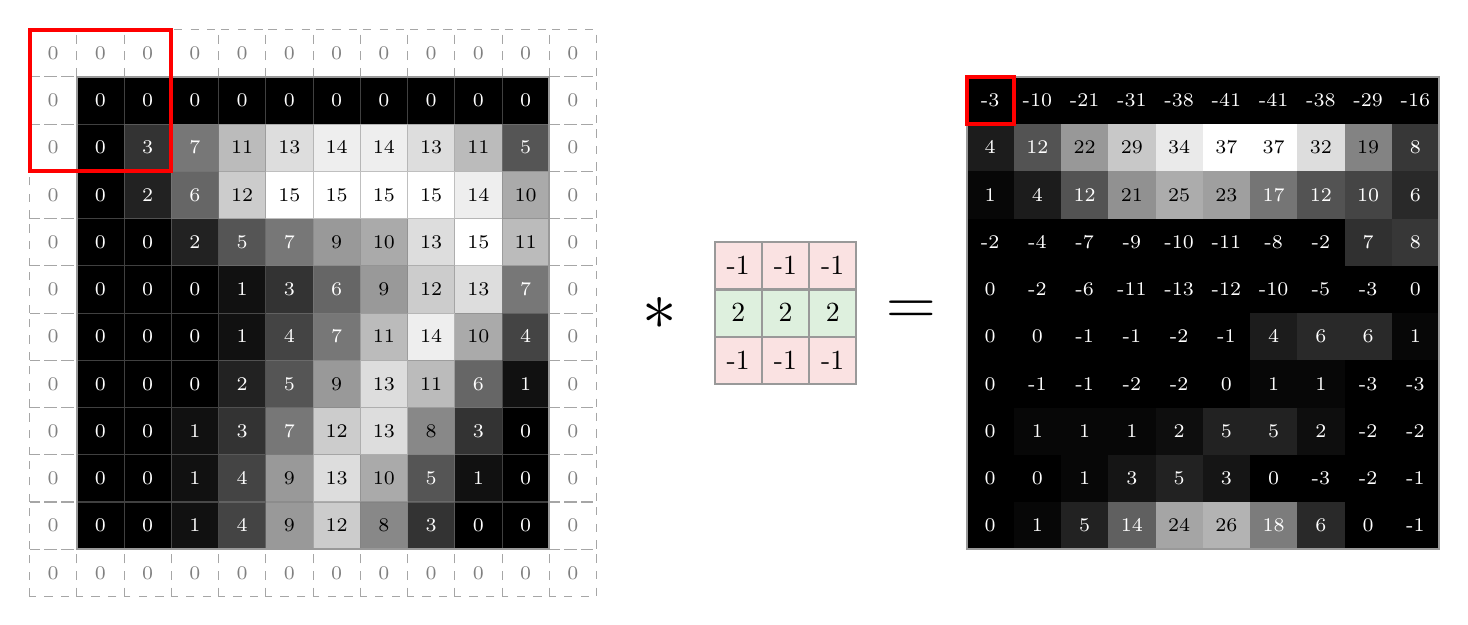
\begin{tikzpicture}[>={Stealth[length=4pt]}, line width=0.8pt, font=\large]

  % ========== 可复用：带数字的 10x10 图（格 0.6，#1 = y 偏移） ==========
  \newcommand{\drawimage}[1]{%
    \foreach \v [count=\n] in {%
      0,0,0,0,0,0,0,0,0,0,%
      0,3,7,11,13,14,14,13,11,5,%
      0,2,6,12,15,15,15,15,14,10,%
      0,0,2,5,7,9,10,13,15,11,%
      0,0,0,1,3,6,9,12,13,7,%
      0,0,0,1,4,7,11,14,10,4,%
      0,0,0,2,5,9,13,11,6,1,%
      0,0,1,3,7,12,13,8,3,0,%
      0,0,1,4,9,13,10,5,1,0,%
      0,0,1,4,9,12,8,3,0,0%
    }{%
      \pgfmathtruncatemacro{\col}{int(mod(\n-1,10))}
      \pgfmathtruncatemacro{\row}{int((\n-1)/10)}
      \pgfmathsetmacro{\gpct}{\v/15}
      \definecolor{px}{gray}{\gpct}
      \fill[px] ({0.6*\col}, {#1+0.6*(9-\row)}) rectangle ++(0.6,0.6);
      \ifnum\v>7 \def\tc{black}\else \def\tc{white}\fi
      \node[font=\scriptsize, text=\tc] at ({0.6*\col+0.3}, {#1+0.6*(9-\row)+0.3}) {\v};
    }
    \begin{scope}[shift={(0,#1)}]
      \draw[gray, opacity=0.5, thin, step=0.6] (0,0) grid (6,6);
      \draw[gray!80] (0,0) rectangle (6,6);
    \end{scope}
  }

  % ========== 可复用：3x3 卷积核 ==========
  \newcommand{\drawkernel}[2]{%
    \foreach \w [count=\m] in {-1,-1,-1,2,2,2,-1,-1,-1} {%
      \pgfmathtruncatemacro{\kc}{int(mod(\m-1,3))}
      \pgfmathtruncatemacro{\kr}{int((\m-1)/3)}
      \ifnum\w>0 \definecolor{kw}{RGB}{222,240,222}\else \definecolor{kw}{RGB}{250,226,226}\fi
      \fill[kw] ({#1+0.6*\kc}, {#2+0.6*(2-\kr)}) rectangle ++(0.6,0.6);
      \node[font=\normalsize] at ({#1+0.6*\kc+0.3}, {#2+0.6*(2-\kr)+0.3}) {\w};
    }
    \begin{scope}[shift={(#1,#2)}]
      \draw[gray!80, step=0.6] (0,0) grid (1.8,1.8);
      \draw[gray!80] (0,0) rectangle (1.8,1.8);
    \end{scope}
  }

  % ========== 可复用：NxN 结果灰度图（全填充，#1 = 宽度 N） ==========
  \newcommand{\drawresultfull}[4]{%
    \foreach \v [count=\n] in {#4} {%
      \pgfmathtruncatemacro{\r}{int((\n-1)/#1)}
      \pgfmathtruncatemacro{\c}{int(mod(\n-1,#1))}
      \pgfmathsetmacro{\g}{max(0, min(\v/37, 1))}
      \definecolor{oc}{gray}{\g}
      \ifdim\g pt>0.5pt \def\tc{black}\else \def\tc{white}\fi
      \fill[oc] ({#2+0.6*\c}, {#3+0.6*(#1-1-\r)}) rectangle ++(0.6,0.6);
      \node[font=\scriptsize, text=\tc] at ({#2+0.6*\c+0.3}, {#3+0.6*(#1-1-\r)+0.3}) {\v};
    }%
    \draw[gray!80] (#2,#3) rectangle ({#2+0.6*#1}, {#3+0.6*#1});
  }

  % ================= zero padding = 1，输出 10x10 =================
  % padding 虚线圈（一圈 0，格子里填 0）
  \foreach \i in {0,...,11} {
    \draw[gray!70, dashed, line width=0.4pt] ({0.6*\i},4.9) rectangle ++(0.6,0.6);
    \node[gray, font=\scriptsize] at ({0.6*\i+0.3},5.2) {0};
    \draw[gray!70, dashed, line width=0.4pt] ({0.6*\i},-1.7) rectangle ++(0.6,0.6);
    \node[gray, font=\scriptsize] at ({0.6*\i+0.3},-1.4) {0};
  }
  \foreach \j in {0,...,9} {
    \draw[gray!70, dashed, line width=0.4pt] (0,{-1.1+0.6*\j}) rectangle ++(0.6,0.6);
    \node[gray, font=\scriptsize] at (0.3,{-0.8+0.6*\j}) {0};
    \draw[gray!70, dashed, line width=0.4pt] (6.6,{-1.1+0.6*\j}) rectangle ++(0.6,0.6);
    \node[gray, font=\scriptsize] at (6.9,{-0.8+0.6*\j}) {0};
  }
  % 原图（右移 0.6）+ 左上角红框（窗口可以盖到 padding 上）
  \begin{scope}[xshift=0.6cm]
    \drawimage{-1.1}
  \end{scope}
  \draw[red, line width=1.4pt] (0,3.7) rectangle (1.8,5.5);

  \node[font=\Huge] at (8.0,1.9) {$\ast$};
  \drawkernel{8.7}{1.0}
  \node[font=\Huge] at (11.2,1.9) {$=$};
  % 完整 10x10 输出（真实计算值）
  \drawresultfull{10}{11.9}{-1.1}{%
    -3,-10,-21,-31,-38,-41,-41,-38,-29,-16,%
    4,12,22,29,34,37,37,32,19,8,%
    1,4,12,21,25,23,17,12,10,6,%
    -2,-4,-7,-9,-10,-11,-8,-2,7,8,%
    0,-2,-6,-11,-13,-12,-10,-5,-3,0,%
    0,0,-1,-1,-2,-1,4,6,6,1,%
    0,-1,-1,-2,-2,0,1,1,-3,-3,%
    0,1,1,1,2,5,5,2,-2,-2,%
    0,0,1,3,5,3,0,-3,-2,-1,%
    0,1,5,14,24,26,18,6,0,-1}
  % 结果图左上角红框（对应左图红框窗口的输出）
  \draw[red, line width=1.4pt] (11.9,4.3) rectangle (12.5,4.9);
\end{tikzpicture}
\end{document}